\section{Setting and hypotheses}\label{sec:setting}

\subsection{Captive spin-offs and the 2022 reform}\label{sec:captive}

A \captive{} changes nothing in the consolidated accounts and nothing in the parent's ownership. Its consequences arrive when the parent's board decides what to do with the subsidiary it now wholly owns---keep it, sell part or all of it, or list it---each a board decision taken without a vote of the parent's shareholders, who afterwards receive their share of any proceeds only insofar as the parent's value reflects them \cite{kang2025}. The objection raised in 2020--2022 had two parts: the loss to the minority occurs at the disposal rather than at the division, and the controlling owner knows at the division more about the disposal than the filing lets the public know. The regulator's three measures answer the two parts with three instruments \cite{fsc2022a, fsc2022b}. The revised disclosure form (18 October 2022) requires the filing to state the division's specific purpose, its expected effects and the measures the company will take to protect its shareholders, and to disclose any plan to list the new company. The appraisal right (late December 2022) lets a shareholder who votes against a \captive{} sell the shares to the company at a price fixed by the pre-announcement market: the mean of the volume-weighted average prices over the two months, one month and one week before the board resolution.\footnote{Article 165-5(3) of the Capital Markets Act and Article 176-7(3) of its enforcement decree \cite{fsc2022b}; a dissenting shareholder who disputes the price may ask a court to set it.} The listing review (28 September 2022) lets the Korea Exchange examine how the parent protected its general shareholders when a carved-out subsidiary applies to list within five years, and refuse the listing. Equity spin-offs---whose choice against the captive form \citeA{kang2025a} analyse---were touched by none of the three. Two features make the setting a laboratory: the disposal is a discrete event the parent must report, so the controller's revealed intention can be measured for every division from public filings; and the filing is a long structured document, so what a reader could have inferred at the announcement can be measured too.

\subsection{Theory}\label{sec:theory}

Four strands of theory meet in a \captive{}. The principal--principal frame \cite{young2008} locates the governance problem of concentrated-ownership firms in the conflict between controlling and minority owners. Korean controllers hold the parent through pyramids and cross-holdings, so their cash-flow stake is often far below their control \cite{laporta1999, claessens2000}; a transfer of value out of the parent costs them only their cash-flow share of the loss while the gain, where it accrues elsewhere in the group, is theirs in full \cite{johnson2000, claessens2002, masulis2011}, and Korean groups have been the canonical setting \cite{bae2002, baek2006, bae2008, joh2003, almeida2011}. A \captive{} is, in this frame, a transfer waiting to happen: it changes the set of decisions the controller can take without the minority.

The economics of disclosure is the second strand, and it is what makes the intention measurable. The filing has two audiences: the minority who vote on the division, and the investors, buyers and listing authorities the controller will need for a disposal, who read the same document. Statements addressed to counterparties are the kind cheap-talk theory classifies as informative---costly to reverse and verifiable after the fact \cite{crawford1982, farrell1996}---where a general statement of purpose (``specialisation'') is not; the information-asymmetry theory of divestitures makes the same point for the US carve-out, which is accompanied by disclosure addressed to the investors who will fund it \cite{nanda1991, krishnaswami1999}; and a voluntary commitment that binds the controller, such as a charter clause requiring a shareholder vote before any listing, is a bonding device \cite{jensen1976}, informative because it is costly. Limited attention is the third strand \cite{hirshleifer2003, dellavigna2009}: investors process the salient part of a disclosure, and the implications of a long document reach prices when the event they foreshadow occurs. The fourth is the economics of mandated disclosure and of shareholder remedies: mandates change what is written, because compliance is cheap and verifiable, and rarely what is done, because the recipients do not read or cannot act \cite{benshahar2014}; an appraisal right is a put on the pre-announcement price \cite{jiang2016}; an ex ante listing review is a deterrent whose force depends on the probability that the disposal takes the reviewed form.

\subsection{Hypothesis 1: the filing is legible}\label{sec:h1}

\emph{Premise.} The principal--principal frame taken alone predicts that the filing should tell the minority nothing: a controller who intends to transfer value has no reason to announce it, and the filing is written to a form. \emph{Mechanism.} The disclosure strand predicts otherwise. A controller who intends to list or sell the subsidiary needs counterparties, and must describe the new company as a vehicle for outside capital, mention a listing application, name a buyer or state investment attraction as a purpose; a controller who intends to keep it has no such need. The informative content lies in verifiable, counterparty-addressed statements, not in the purpose categories a form elicits from every filer. \emph{Boundary.} The filing can be informative only about intentions that exist at the announcement; disposals decided years later for reasons that arose later are noise against which any reader, human or machine, will fail, so the signal should be sharpest for disposals that follow quickly. \emph{Rival.} Under the boilerplate view a reading of the text predicts the disposal no better than the parent's financial position, and no better than the coarse purpose categories that \citeA{kang2025} hand-coded for this population; under the cheap-talk view the purpose categories carry the information and a holistic reading adds nothing to them.

\textbf{H1.} A reading of the division filing predicts whether the subsidiary is later disposed of, and does so beyond the financial characteristics stated in the filing and beyond its stated-purpose categories and mention flags; the increment is largest for disposals within a year of the division.

\subsection{Hypothesis 2: the controlling owner's stake}\label{sec:h2}

\emph{Premise.} If divisions were decided on the subsidiary's merits---the efficiency view of divestitures, in which the division is a refocusing or financing device \cite{krishnaswami1999, slovin1995, powers2003, vijh2002}---the controller's stake would have nothing to do with the disposal. \emph{Mechanism.} The principal--principal arithmetic says otherwise: the controller's gain from a disposal does not depend on the controller's cash-flow stake in the parent, while the controller's share of the parent's loss does, so a smaller stake lowers the private cost of a disposal and raises the probability that the division is undertaken with one in view. If H1 holds, that intention is legible, so the stake should predict the signal as well as the outcome. \emph{Boundary.} The stake is one determinant among several---a controller with a large stake may dispose because the subsidiary needs capital the parent cannot supply, a controller with a small stake may retain because the subsidiary is the group's core---so the prediction concerns the direction of an association, and we measure the stake as the parent reports it, which overstates the family's cash-flow right where affiliates hold much of the block. \emph{Rival.} Under the efficiency view the block is unrelated to the signal and to the disposal.

\textbf{H2.} The smaller the controlling block before the announcement, the stronger the disposal signal in the filing and the more likely the subsidiary is disposed of; the block's association with the disposal runs through the signal.

\subsection{Hypothesis 3: the market}\label{sec:h3}

\emph{Premise.} Under semi-strong efficiency minority investors read the filing as a careful reader would: a filing that signals a disposal is met with a weaker or more negative announcement return, and nothing systematic follows, because the loss is in the price at the announcement. \emph{Mechanism of the rival.} Under limited attention investors react to the salient content---a growth story about outside capital and a listing---and the implications buried in the document reach prices when the disposal occurs, so the announcement return is unrelated or positively related to the signal, and the subsequent return falls with the signal and with the realised disposal, most steeply where the disposal comes quickly and where the controlling block is small. \emph{Boundary.} The test requires a signal measurable at the announcement (H1), a window that captures the disposals that follow quickly, benchmarks that do not load on size or value, and controls for the parent's condition, since a troubled parent might both write a filing that reads as a disposal and go on to underperform. \emph{Rival.} The efficient-reading prediction is the hypothesis; the limited-attention pattern is the alternative, stated in full so that the evidence can choose.

\textbf{H3.} (a) The announcement return is lower where the filing signals a disposal, and (b) the return over the following year is unrelated to the signal; under the rival, (a$'$) the announcement return is unrelated or positively related to the signal, (b$'$) the following year's return falls with the signal and the loss arrives with the realised disposal, and (c$'$) the loss falls on the minority holders of small-block parents.

\subsection{Hypothesis 4: the reform's three channels}\label{sec:h4}

The regulator's description implies one prediction for all three measures: they deter disposal-oriented divisions, so that post-reform filings signal disposal less and early disposal is rarer. The fourth strand separates the measures by the channel through which each acts.

\emph{Information channel (H4a).} \emph{Premise:} the mandate is addressed to shareholders who, under the limited-attention rival of H3, were not reading the filing. \emph{Mechanism:} compliance is cheap and verifiable, so the statements appear at once and the reception of the filing---now a document that states protection---improves, while the controller's intention, which the mandate does not touch, does not. \emph{Boundary:} a before-and-after comparison confounds the mandate with the market of 2023--2026; equity spin-offs, filed under the same conditions but exempt from the reform, provide the difference. \emph{Rival:} the deterrence view predicts a weaker signal and a smaller reaction. \textbf{H4a.} Relative to equity spin-offs, the announcement reaction to a \captive{} rises after October 2022 while the disposal signal does not fall.

\emph{Compensation channel (H4b).} \emph{Premise:} the appraisal right fixes a strike at the price prevailing before the announcement. \emph{Mechanism:} for a shareholder who dissents it is a put; its value at the announcement is its moneyness, the appraisal price relative to the current price, and a market that prices rights should price it, so the announcement return of post-reform \captive{}s should rise with moneyness. \emph{Boundary:} the right exists only for \captive{}s after December 2022 and only for dissenters; before the reform, and for equity spin-offs, the same price ratio can be computed from the decree's formula but carries no right. \emph{Rival:} if the right is not exercised or not priced, the slope is zero in all three samples. \textbf{H4b.} The announcement return of post-reform \captive{}s increases with the moneyness of the appraisal price; the same ratio has no slope for pre-reform \captive{}s or for equity spin-offs.

\emph{Deterrence and bonding channel (H4c).} \emph{Premise:} the listing review raises the cost of the disposal's most valuable form, and the revised form invites the parent to state how it will protect shareholders. \emph{Mechanism:} a parent that intends to keep the subsidiary can say so at no cost in a way that binds---a charter clause requiring a shareholder vote before any listing, a stated horizon without listing---while a parent that intends to dispose cannot afford to; the content of the protection block, not its presence, therefore separates intentions \cite{jensen1976, farrell1996}. \emph{Boundary:} the block is mandatory, so its presence is uninformative; the post-reform sample is small and its outcomes young. \emph{Rival:} under the cheap-talk view of mandated statements \cite{benshahar2014} the block's content is unrelated to the signal and to realised disposal. \textbf{H4c.} Among post-reform filings, those whose protection block commits the parent carry a lower disposal signal and dispose less often than those that recite the form.

Figure~\ref{fig:framework} places the hypotheses on the two steps of the transaction, and Table~\ref{tab:hyp} lists, for each, the prediction, its rival and the test that decides between them.

\begin{figure}[htbp]
\centering
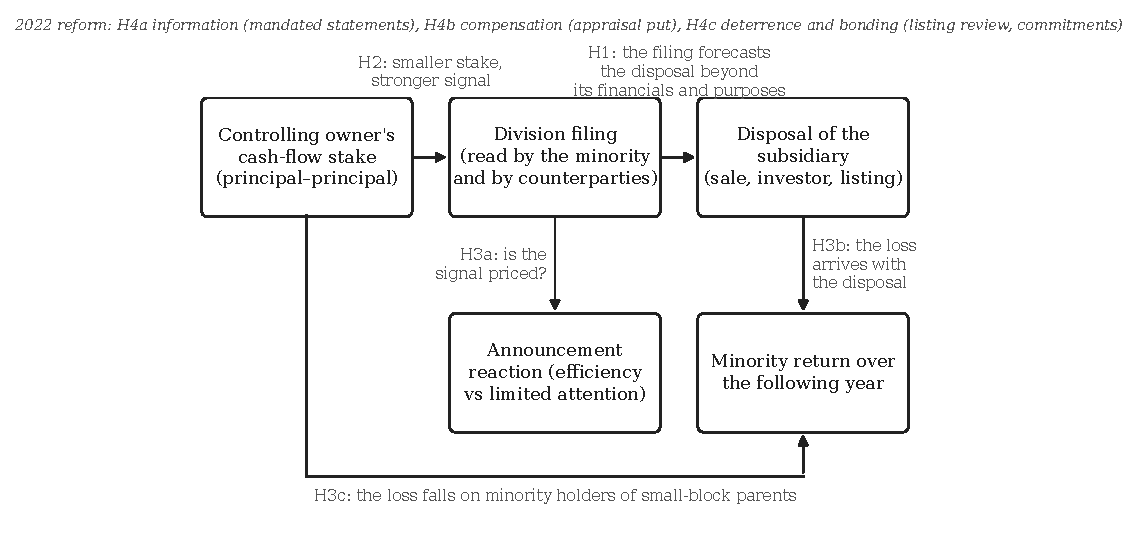
\includegraphics[width=\textwidth]{../figures/F1_framework_jifma.pdf}
\caption{The two steps of a \captive{} and the hypotheses}\label{fig:framework}
\tabnote{Boxes are the quantities the paper measures; arrows carry the hypotheses of Section~\ref{sec:setting}. H1 and H2 concern what the filing reveals and why; H3 concerns how the market and the minority's returns respond; H4a--c concern the three channels of the 2022 reform.}
\end{figure}

\begin{table}[htbp]
\centering
\caption{Hypotheses, rival predictions and tests}\label{tab:hyp}
{\scriptsize\singlespacing\setlength{\tabcolsep}{4pt}
\begin{tabular}{>{\raggedright\arraybackslash}p{1.5cm}>{\raggedright\arraybackslash}p{4.1cm}>{\raggedright\arraybackslash}p{3.7cm}>{\raggedright\arraybackslash}p{4.4cm}}
\toprule
Hypothesis & Prediction (theory) & Rival prediction & Test and exhibit \\
\midrule
H1 legibility & Filing text predicts disposal beyond financials and purpose categories; sharpest for early disposals (disclosure economics, verifiable statements) & No increment over financials (boilerplate) or over purpose categories (cheap talk) & Nested cross-validated models M0--M3 with bootstrap increments; Cox hazard with period strata; Table~\ref{tab:gate1}, Fig.~S1 \\
H2 stake & Smaller block $\rightarrow$ stronger signal, more disposals; block acts through the signal (principal--principal) & Block unrelated to signal and disposal (efficiency view) & Signal and disposal on the block with year, industry FE, firm clusters, foreign ownership, board; Table~\ref{tab:block} \\
H3 market & (a) lower announcement return and (b) no drift where the filing signals disposal (efficiency) & (a$'$) non-negative reaction, (b$'$) drift that arrives with the disposal, (c$'$) concentrated in small-block parents (limited attention) & Announcement CAR and one-year rank on the signal; benchmarks, FE, clusters, controls; realised early disposal; Table~\ref{tab:returns}, Fig.~\ref{fig:signal} \\
H4a information & Reaction rises relative to equity spin-offs; signal unchanged (mandated disclosure) & Signal falls, reaction falls (deterrence) & Captive $\times$ post DiD against equity spin-offs with placebo cut; Table~\ref{tab:reform}, Panel A \\
H4b compensation & Reaction rises with appraisal-price moneyness for post-reform captives only (put) & No slope anywhere (right not priced) & CAR on moneyness with pre-reform and equity-spin-off placebos; Table~\ref{tab:reform}, Panel C \\
H4c deterrence, bonding & Binding protection statements carry lower signal and fewer disposals (bonding) & Content unrelated to signal and disposal (cheap talk) & Protection-block categories and strength against the signal and labelled disposals; Table~\ref{tab:reform}, Panel B \\
\bottomrule
\end{tabular}}
\end{table}
